\documentclass[11pt,twocolumn,twoside]{extarticle}

\usepackage[utf8]{inputenc}
\usepackage[T1]{fontenc}
\usepackage[letterpaper,top=1.85cm,bottom=1.7cm,left=1.55cm,right=1.55cm,columnsep=0.62cm,headheight=14pt,headsep=8pt]{geometry}
\usepackage{newtxtext}
\usepackage[scaled=0.92]{helvet}
\usepackage{placeins}
\usepackage{fontawesome5}
\usepackage{orcidlink}
\hypersetup{colorlinks=true,urlcolor=black,linkcolor=black,citecolor=black}
\usepackage{microtype}
\usepackage{graphicx}
\usepackage{booktabs}
\usepackage{array}
\usepackage{ragged2e}
\usepackage{tabularx}
\usepackage{caption}
\usepackage{titlesec}
\usepackage{dblfloatfix}
\usepackage[superscript]{cite}
\usepackage{url}
\usepackage{fancyhdr}

\frenchspacing
\hyphenation{figure}
\setcounter{secnumdepth}{0}
\titleformat{\section}{\sffamily\bfseries\fontsize{13}{16}\selectfont}{}{0pt}{}
\titleformat{\subsection}{\sffamily\bfseries\normalsize}{}{0pt}{}
\titleformat{\subsubsection}{\bfseries\normalsize}{}{0pt}{}
\titlespacing*{\section}{0pt}{1.15ex plus 0.2ex}{0.45ex}
\titlespacing*{\subsection}{0pt}{0.95ex plus 0.2ex}{0.3ex}
\titlespacing*{\subsubsection}{0pt}{0.75ex plus 0.2ex}{0.2ex}

\DeclareCaptionLabelSeparator{pipe}{\,\textbar\,}
\captionsetup{
  font=small,
  labelfont={bf,sf},
  labelsep=pipe,
  skip=3pt,
  justification=justified,
  singlelinecheck=false
}
\captionsetup[figure]{name=Fig.}
\captionsetup[table]{name=Table,position=top}

\makeatletter
\renewcommand\@biblabel[1]{#1.}
\makeatother

\pagestyle{fancy}
\fancyhf{}
\fancyhead[LE,RO]{\footnotesize\thepage}
\fancyhead[LO]{\footnotesize\textit{Inhibiting LINE-1 in disease}}
\renewcommand{\headrulewidth}{0.3pt}
\fancypagestyle{plain}{%
  \fancyhf{}%
  \fancyhead[LE,RO]{\footnotesize\thepage}%
  \fancyhead[LO]{\footnotesize\textit{Inhibiting LINE-1 in disease}}%
  \renewcommand{\headrulewidth}{0.3pt}%
}

\renewcommand{\topfraction}{0.92}
\renewcommand{\bottomfraction}{0.6}
\renewcommand{\textfraction}{0.06}
\renewcommand{\floatpagefraction}{0.75}
\renewcommand{\dbltopfraction}{0.92}
\renewcommand{\dblfloatpagefraction}{0.65}
\setcounter{topnumber}{3}
\setcounter{dbltopnumber}{2}
\setlength{\emergencystretch}{2.5em}
\clubpenalty=8000
\widowpenalty=8000

\newcolumntype{Y}{>{\raggedright\arraybackslash}X}

\begin{document}
\twocolumn[%
{\sffamily\bfseries\fontsize{15.5}{18.5}\selectfont
Inhibiting LINE-1 retrotransposons therapeutically in disease\par}
\vspace{0.55em}
{\normalsize William Brandler$^{1}$\,\orcidlink{0000-0001-5280-325X}\par}
\vspace{0.25em}
{\small $^{1}$L1 Therapeutics, william{\char64}l1tx.com\par}
\vspace{0.35em}
{\normalsize\today\par}
\vspace{0.65em}
\setlength{\fboxsep}{8pt}%
\setlength{\fboxrule}{0.6pt}%
\noindent\fbox{\begin{minipage}{\dimexpr\textwidth-2\fboxsep-2\fboxrule\relax}
{\sffamily\bfseries Abstract}\par\vspace{0.35em}
The LINE-1 retrotransposon is a virus-like genomic element that can activate in diseased cells. It has been implicated in cancer, autoimmunity, developmental disorders, infectious disease and neurodegeneration. LINE-1 can be inhibited by reverse transcriptase inhibitors, small molecules originally developed for HIV. The correlation between HIV and LINE-1 inhibition is $\sim$0.9 on a log scale, in spite of $>$450\,Mya of evolutionary history since retroviruses diverged from retrotransposons. Suppression of HIV requires prevention of a completed 9.7\,kb virus insertion into the genome in immune cells. However, every cell in the body already contains $>$100 copies of LINE-1 that can potentially activate. Even incomplete LINE-1 mediated insertions can cause damaging mutations and genome instability. Furthermore, partial HIV and LINE-1 products in the cytoplasm of cells can contribute to an inflammatory immune response. Preclinical studies have shown LINE-1 inhibitors slow the progression of otherwise unrelated diseases. LINE-1's contribution to these diseases can potentially be quantified using single-nucleus whole-genome sequencing on diseased tissue, enabling prioritization of disease selection for therapeutic development. Furthermore, LINE-1's ORF1p protein can be measured in the blood of individuals with certain cancers. LINE-1 inhibitors could therefore be extended to various diseases. Potentially used both as an anti-inflammatory and prophylactically to help preserve genome integrity. Reverse transcriptase inhibitors are available at low cost for HIV, and higher doses of some could be used to inhibit LINE-1. However, reverse transcriptase inhibitors do not prevent DNA cutting by LINE-1's endonuclease. Novel inhibitors may therefore be required. This, combined with novel diagnostics, opens up possibilities for inhibiting LINE-1 therapeutically in disease
\end{minipage}}
\vspace{1.05em}
]

\section{Introduction}
One of the biggest impacts on the genome structure and evolution has been retrotransposons. These are virus-like elements that copied and spread over evolutionary time, accounting for $\sim$43\% of the human genome. They also activate under stress in many diseases. This triggers the innate immune system to raise an inflammatory antiviral response, known as `viral mimicry' (De Cecco et al., 2019). This can contribute to both autoimmunity and immune evasion in cancer (You et al., 2025). They further create genomic instability, which can contribute to both cancer and degeneration (Rodriguez-Martin et al., 2020; Gasior et al., 2006). Retrotransposons are suppressed in healthy cells

The research article below will explain what retrotransposons are and how they can be targeted therapeutically

\section{Evolution of Retrotransposons}
Retrotransposons evolved from bacterial group II introns over 1 billion years ago. They are near universal across eukaryotes. However, the naked mole rat, a relatively long-lived species in a highly stable environment with low predation, has lost retrotransposition competent elements (Ivancevic et al., 2016). Although LINE-1 has gone extinct in some other mammalian species (Ivancevic et al., 2016), perhaps through selection or genetic drift, mice contain $>$2,000 copies of active elements (Goodier et al., 2001). Retroviruses such as HIV evolved from retrotransposon-like precursors, also using reverse transcriptase (RT) to copy their RNA into host genomes (Figure~\ref{fig:genomes}A)

\section{LINE-1 in humans}
Most retrotransposons in the human genome have been inactivated by mutation, but $>$100 copies of the LINE-1 retrotransposon are still capable of copying themselves (Yang et al., 2024). LINE-1 copies itself but also other sequences that hijack its machinery, which has resulted in almost half the genome consisting of retrotransposon derived sequences. LINE-1 itself accounts for $\sim$17\% of the human genome in $\sim$500,000 copies. Active elements are $\sim$6\,kb and encode two proteins, ORF1p and ORF2p (Figure~\ref{fig:genomes}A). ORF1p binds to LINE-1 messenger RNA, and ORF2p cuts DNA and reverse transcribes (copies) LINE-1 mRNA back into genomic DNA. This reverse transcription process can occur in the cytoplasm of the cell, producing complementary DNA (Baldwin et al., 2024), which triggers the defense response to viruses initiated by the cell (De Cecco et al., 2019). When DNA is abundant in the cytoplasm this can begin at 45\,bp (Andreeva et al., 2017), and at 60\,bp for an RNA:DNA hybrid (which is what LINE-1 produces when reverse transcribing) (Mankan et al., 2014). Longer sequences trigger inflammation more efficiently (Du and Chen, 2018). At the amount of DNA present in an infection, the response can require a few hundred base pairs (Luecke et al., 2017)

There are two types of retrotransposition, classical \& non-classical (Figure~\ref{fig:genomes}B). Classical retrotransposition results in an insertion with a polyA tail (from the messenger RNA of LINE-1 or hijacked sequence). Insertions often contain target-site duplications (TSD). Non-classical retrotransposition involves no polyA, no TSD, and is truncated at both ends (3$'$ and 5$'$). Non-classical is independent of endonuclease (ENi), relying only on reverse transcriptase (Morrish et al., 2002). ENi events have been observed in the brain (Jacob-Hirsch et al., 2018), particularly in certain diseases such as Ataxia-Telangiectasia and Tuberous Sclerosis, but have not (yet) been seen in cancer

\begin{figure*}[!t]
{\raggedright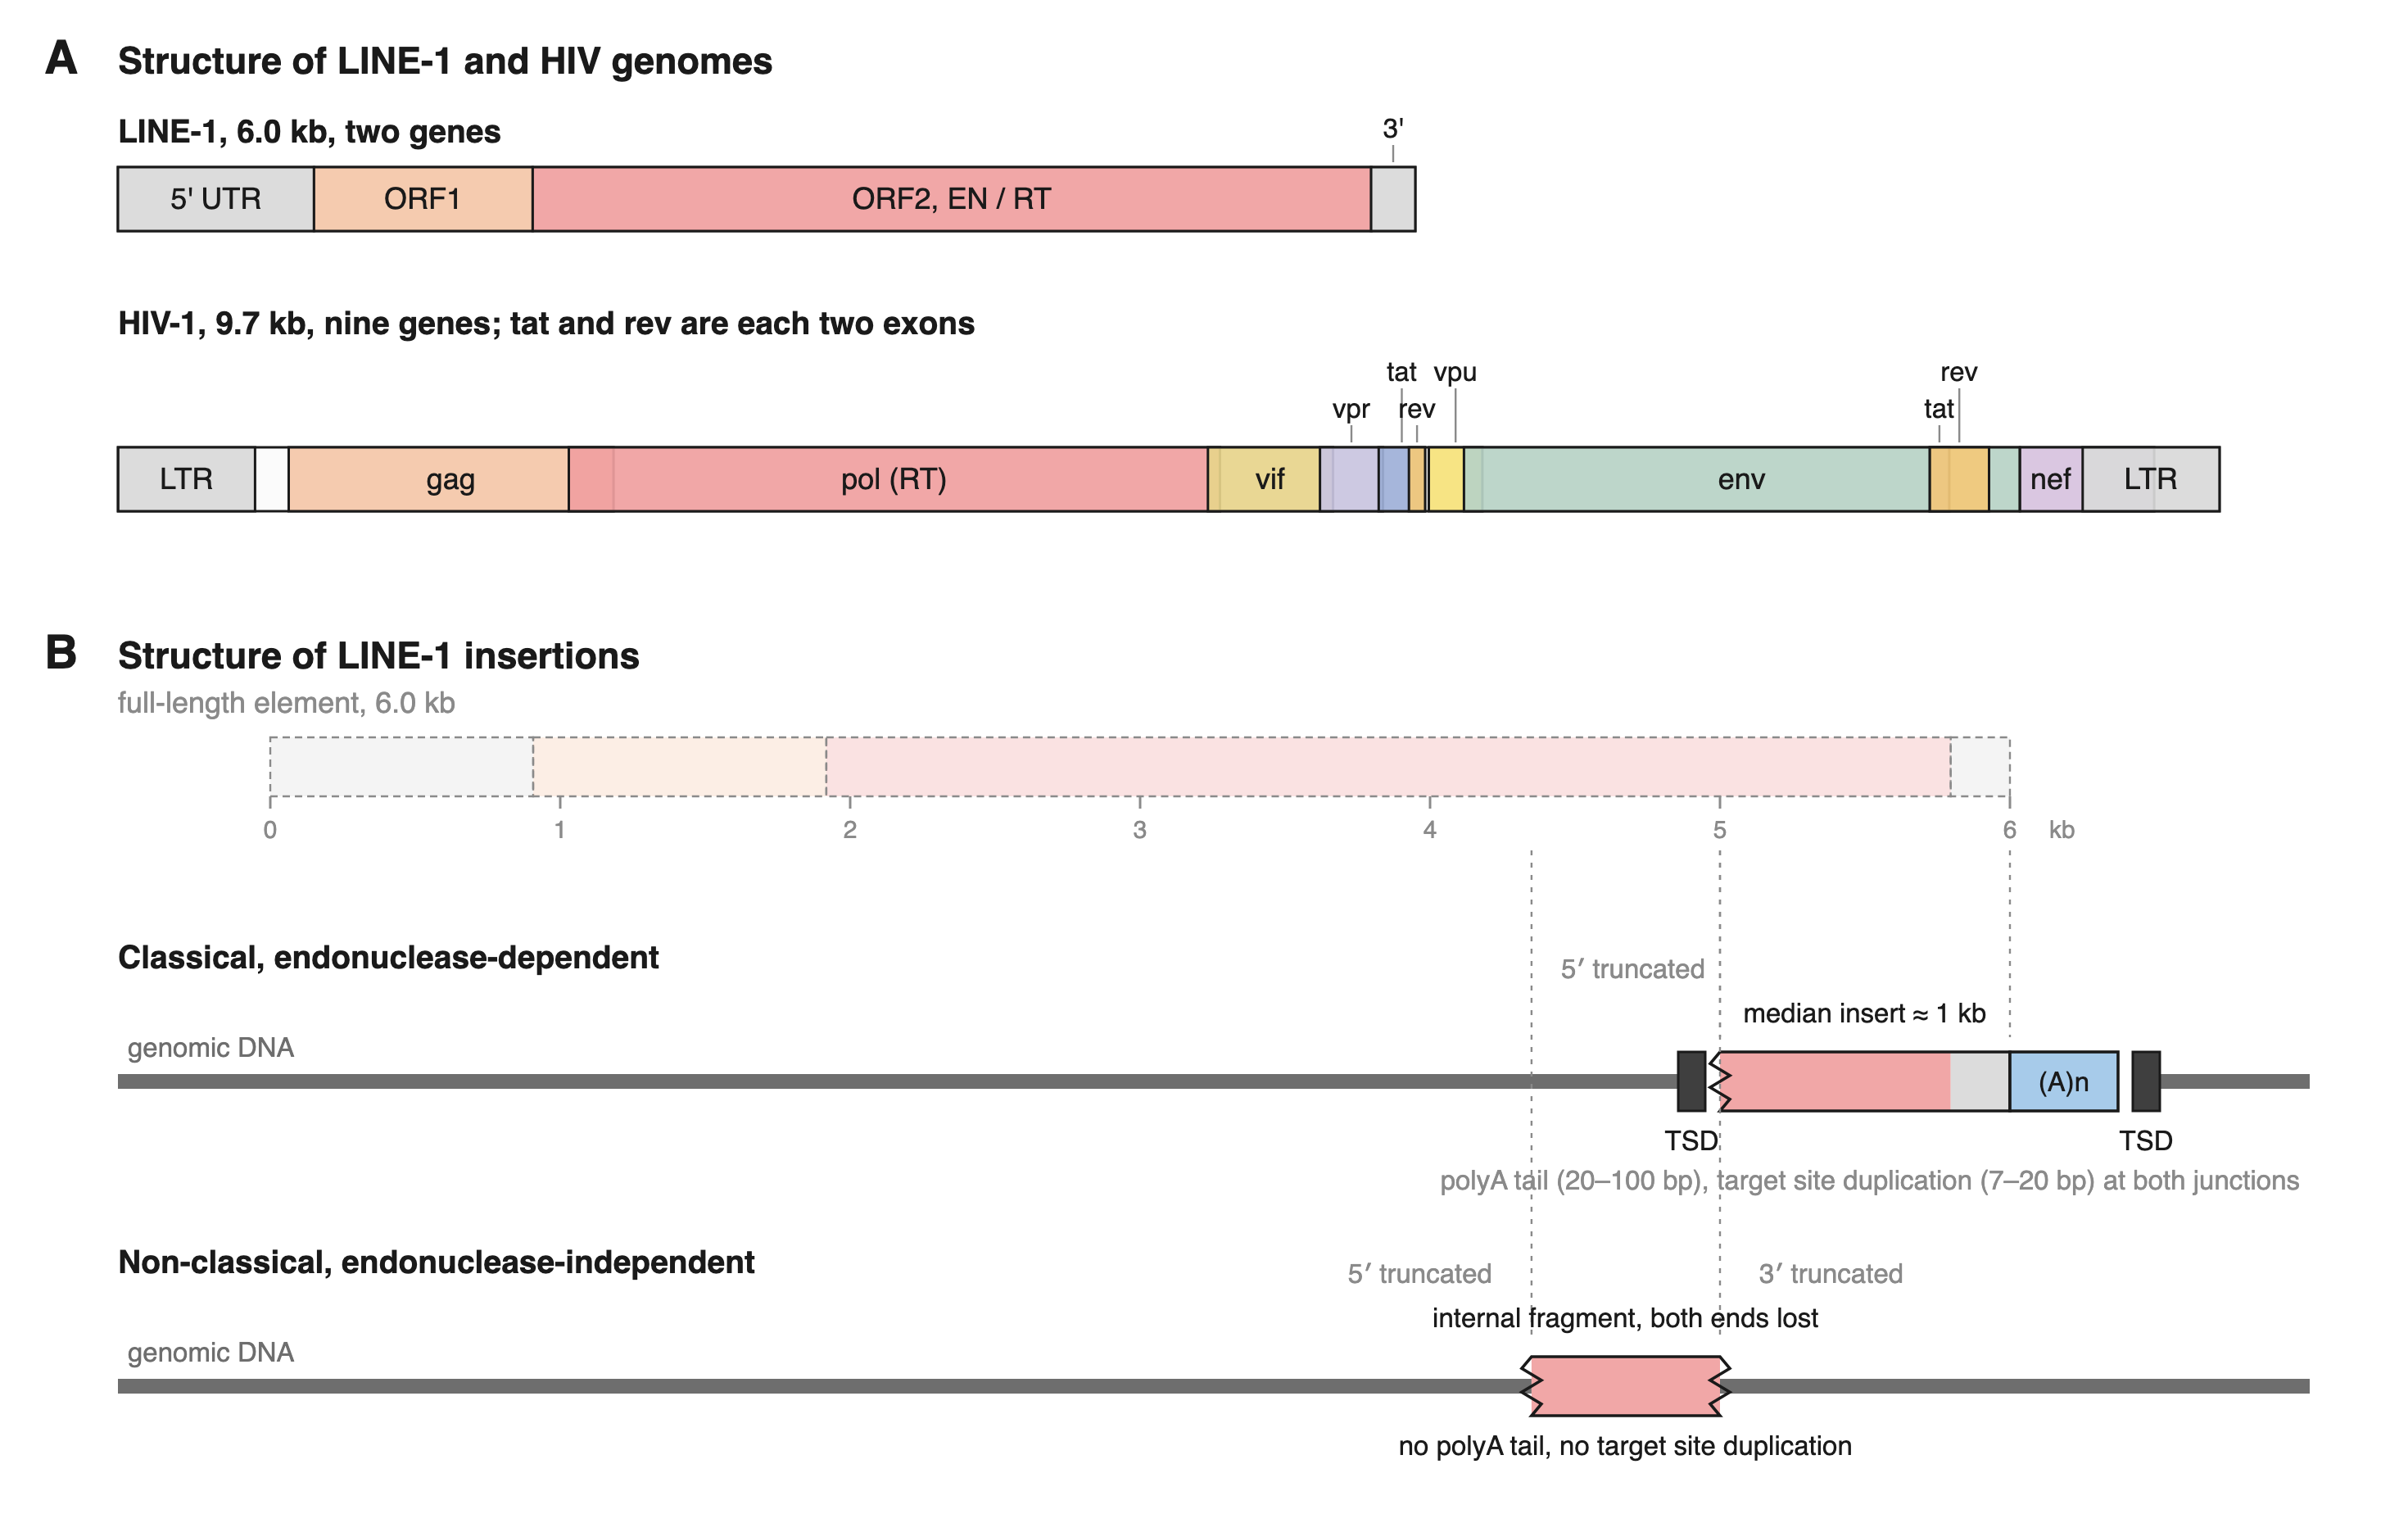
\includegraphics[width=0.77\textwidth]{../genomes.png}\par}
\caption{\textbf{Genome structure and insertion classes for LINE-1 and HIV-1}
\textbf{a}, LINE-1 is 6.0\,kb and encodes ORF1p and ORF2p (endonuclease and reverse transcriptase). HIV-1 is 9.7\,kb; reverse transcriptase is in \textit{pol}.
\textbf{b}, Classical, endonuclease-dependent insertions are usually 5$'$ truncated and retain a polyA tail and target-site duplications. Non-classical, endonuclease-independent insertions are truncated at both ends}
\label{fig:genomes}
\end{figure*}

LINE-1 can also disrupt the functions of genes and contribute to genome instability. Successful insertions in the sense orientation of genes inside their introns can introduce cryptic splice sites, polyadenylation signals, or otherwise impact gene expression (Perepelitsa-Belancio and Deininger, 2003). Insertions in the population are depleted in introns in a sense orientation relative to genes. Modeled from this, new retrotransposon insertions contribute roughly 5--14\% of new loss-of-function gene mutations per birth. Furthermore, insertions inside exons of genes disrupt the gene completely (Cajuso et al., 2019). Failed insertions leave a scar of small insertion/deletion events (Zhang et al., 2026). They can cause more complex rearrangements such as reciprocal translocations between two chromosomes, or inversions of sequence (Zumalave et al., 2026; Mendez-Dorantes et al., 2026). This genome instability can generate further structural rearrangements such as deletions and duplications, complex rearrangements or DNA fragmentation, which is important in cancer (Mendez-Dorantes et al., 2026). Retrotransposons are not the only factor influencing genome integrity. However, the damage they cause can contribute to both apoptosis and cell death as well as to cancer evolution, as we shall see in later sections

\section{How does LINE-1 contribute to disease?}
LINE-1 is heavily suppressed in healthy adult cells through regulation of gene expression, sensing and degradation of foreign DNA, autophagy and breakdown of ribonucleoproteins, repair of DNA damage, triggering of cell death or apoptosis (Goodier, 2016). Many different diseases involve dysregulation of genes involved in these processes. LINE-1 is typically not the initiating factor of these diseases but is instead a downstream consequence that can contribute to disease progression. The ORF2p protein of LINE-1 is so toxic to cells that scientists were only recently able to produce enough of it to determine its 3D structure (Leslie, 2025). Genome sequencing has revealed elevated levels of LINE-1 insertions into DNA in both cancer and neurological disorders (Rodriguez-Martin et al., 2020; Jacob-Hirsch et al., 2018)

\section{LINE-1's role in disease}
Like many viruses, LINE-1 is both inflammatory and a mutagen. However, everyone contains $>$100 potentially active copies in every cell in the body. Independent studies have implicated LINE-1 in many diseases (Table~\ref{tab:diseases}). These include cancers, autoimmune disorders, developmental disorders, infectious disease and degeneration. The evidence for each disease varies, some have mechanistic explanations, genomic or transcriptomic data, LINE-1 inhibition data, cell line or animal model data, and clinical trial data

\begin{table*}[!t]
\caption{\textbf{Diseases in which LINE-1 has been implicated}}
\label{tab:diseases}
\vspace{0.3em}
\footnotesize
\setlength{\tabcolsep}{4pt}
\renewcommand{\arraystretch}{1.12}
\begin{tabularx}{\textwidth}{@{}>{\RaggedRight\arraybackslash}p{4.15cm} >{\RaggedRight\arraybackslash}p{3.15cm} >{\RaggedRight\arraybackslash}p{2.05cm} Y l@{}}
\toprule
\textbf{Disease} & \textbf{Category} & \textbf{Gene} & \textbf{LINE-1 mechanism} & \textbf{References} \\
\midrule
Senescence & Aging & RB1 & chromatin relaxation; accumulation of L1 cDNA & \cite{cecco} \\
Progeroid syndromes & Aging & LMNA, SIRT6 & accumulation of L1 RNA; chromatin relaxation & \cite{simon,dellavalle} \\
Ataxia-telangiectasia & Neurodevelopmental & ATM & delayed DNA break repairs & \cite{jacob,takahashi,coufal} \\
Rett syndrome & Neurodevelopmental & MECP2 & hypomethylation & \cite{muotri,jacob,martins} \\
Down syndrome & Neurodevelopmental &  & misregulated L1 expression & \cite{martinez,borgognone} \\
Tuberous sclerosis & Neurodevelopmental & TSC1, TSC2 & mTOR growth signaling activates L1 & \cite{jacob,martin} \\
Cytomegalovirus & Infectious & TSC2 & mTOR growth signaling activates L1 & \cite{hwang,park} \\
Aicardi-Gouti\`eres & Inflammatory & TREX1 & accumulation of L1 cDNA & \cite{thomas,crow} \\
Fanconi anemia & Inflammatory & SLX4, FANCD2 & accumulation of L1 cDNA & \cite{bregnard} \\
Sterile inflammation & Inflammatory & CGAS, STING1 & accumulation of L1 cDNA & \cite{cecco} \\
Lupus & Autoimmune &  & demethylation; accumulation of L1 RNA & \cite{mavragani} \\
GI, lung, head \& neck, ovarian & Oncological & TP53 & demethylation & \cite{rodriguez,gasior,zhang,mendez,rajurkar,pisanic} \\
Chemo / radiotherapy & Oncological & TP53 & DNA damage / stress induced activation & \cite{rajurkar} \\
ALS / FTD & Neurodegenerative & TARDBP & chromatin relaxation & \cite{liu} \\
Alzheimer / tauopathy & Neurodegenerative & MAPT & chromatin relaxation & \cite{guo,sun,herdy} \\
Parkinson's & Neurodegenerative &  & L1 activation in substantia nigra and putamen neurons and microglia & \cite{garza,gordillo} \\
Geographic atrophy & Degenerative & DICER1 & L1 reverse transcription of Alu RNA & \cite{fukuda} \\
\bottomrule
\end{tabularx}
\end{table*}

LINE-1 inhibitors have slowed progression of otherwise unrelated diseases in preclinical studies, including cancer (Rajurkar et al., 2022; Novototskaya-Vlasova et al., 2022), progeroid syndromes (Simon et al., 2019; Della Valle et al., 2022), Rett syndrome (Martins et al., 2026), Ataxia-Telangiectasia (Takahashi et al., 2022), Aicardi-Gouti\`eres syndrome (AGS) (Thomas et al., 2017), Down syndrome (Martinez de Lagran et al., 2022), Alzheimer's (Herdy et al., 2026), and non-infectious (sterile) inflammation (De Cecco et al., 2019). The degree to which LINE-1 contributes to any of these diseases is not well established. Studies typically use older reverse transcriptase inhibitors such as Lamivudine (3TC) or Stavudine (d4T), because they are readily available at low cost. Both are much less potent than later inhibitors (Figure~\ref{fig:nrti}A; Table~\ref{tab:nucleosides}). Stavudine also has a narrow therapeutic window due to mitochondrial polymerase $\gamma$ toxicity, but the effect nucleosides have on mitochondria varies substantially (Table~\ref{tab:nucleosides}). Studies using less effective nucleosides may underestimate the potential effects of LINE-1 inhibitors, but they also use continuous high doses that can overestimate their effects

Although LINE-1 inhibition shows promise, it is not yet resolved what the relative contribution of LINE-1 is to each disease. Many studies use indirect methods such as signatures of inflammation or LINE-1 mRNA expression, which are challenging to attribute to elevated retrotransposition accurately (Faulkner, 2023). Whole-genome sequencing has identified elevation of LINE-1 insertions in post-mortem or biopsied brain tissue of individuals with Ataxia-Telangiectasia, Tuberous Sclerosis, and Rett Syndrome (Jacob-Hirsch et al., 2018). It is also controversial how much LINE-1 activation occurs in the brain (Jacob-Hirsch et al., 2018; Upton et al., 2015; Erwin et al., 2016; Evrony et al., 2016). To accurately measure this requires single-nucleus whole-genome sequencing of post-mortem brain tissue. Novel computational biology algorithms are also required, such as retrotransposon-miner (\href{https://github.com/L1-Therapeutics/retrotransposon-miner}{\faGithub}~\url{https://github.com/L1-Therapeutics/retrotransposon-miner})

Another unresolved issue is determining when it is possible to intervene during the course of disease progression. It is possible to measure LINE-1 in real-time in cancer because dying cancer cells release LINE-1 ORF1p protein. However, for neurological disorders or diseases of aging this requires retrospective studies of diseased tissue

Furthermore, LINE-1 is not the only contributor to inflammation. LINE-1 induced cell-death / degeneration cannot be reversed. Also LINE-1 mutations insert unpredictably and are not the only mutagenic factor in cancer or cell death. LINE-1 inhibitors are not necessarily a cure for any disease, however they may be an important piece of the puzzle in some diseases. They would be used as an anti-inflammatory, or prophylactically to preserve genome stability over a period of years. But the long timelines of disease progression make it both costly and challenging to measure benefits in a traditional clinical trial setting

In spite of promising preclinical studies, there have not yet been approvals for reverse transcriptase inhibitors outside of viral infections. Censavudine has been tested in a phase 2 clinical trial against LINE-1 for amyotrophic lateral sclerosis (ALS) (NCT04993755), Lamivudine for colorectal cancer (NCT03144804; Rajurkar et al., 2022), and a combination of inhibitors for Aicardi-Gouti\`eres syndrome (Crow et al., 2025). A phase 1b/2a trial of Lamivudine for Alzheimer's disease in people with Down syndrome was funded by the National Institute on Aging in 2026 and is not yet registered (1UG3AG101657)

\section{Therapeutic Strategies for LINE-1}
Three strategies have been proposed for LINE-1, antisense oligonucleotides (ASOs), ORF2p endonuclease inhibitors and ORF2p reverse transcriptase inhibitors (Della Valle et al., 2022; D'Ordine et al., 2024; Jones et al., 2008; Dai et al., 2011). Other approaches include cancer vaccines against ORF1p (McKerrow et al., 2025). However, they will not be discussed here

\subsection{Reverse transcriptase inhibitors (RTIs)}
Reverse transcriptase inhibitors are analogues of nucleosides, the building blocks of DNA. There are nucleoside inhibitors for adenosine, cytidine, thymidine and guanosine. Over 1,000 nucleoside and nucleoside phosphonate analogues have been tested across antiviral programs \cite{siegel}. For HIV, more than 600 nucleosides have been tested \cite{raheemcroi}. Separately, $>$300 have been tested for LINE-1 activity, and 25 have been tested on both HIV and LINE-1 (Table~\ref{tab:nucleosides}). The potency of RTIs for HIV correlates strongly with their potency for LINE-1 (Figure~\ref{fig:nrti}A). Retroviruses diverged evolutionarily from retrotransposons $>$450\,Mya (Aiewsakun and Katzourakis, 2017). However, both take deoxyribose nucleoside triphosphates (dNTPs) as substrates, which are unchanged since the dawn of life. Consequently, the shape of the active site of the enzyme has been preserved across evolutionary time (Baldwin et al., 2024). This creates a vulnerability that nucleoside chemists have exploited to develop antivirals. Antivirals work consistently on HIV and LINE-1 reverse transcriptases, and some show substantial selectivity over host enzymes that take dNTPs as substrates (such as mitochondrial polymerase gamma, telomerase, and DNA polymerase). However, LINE-1 may require higher dosing to be sufficiently inhibited, and approved HIV regimens are constructed to provide the minimum necessary dose to sufficiently inhibit HIV. Potency is not the only consideration, as molecules that do inhibit LINE-1 / HIV can also have off-target effects (Table~\ref{tab:nucleosides}), cross the blood-brain barrier with varying efficiency, be activated in only certain cell types, or have different half-lives

\begin{figure*}[!t]
\noindent
\begin{minipage}[t]{\textwidth}
{\sffamily\bfseries A}\par\vspace{1pt}
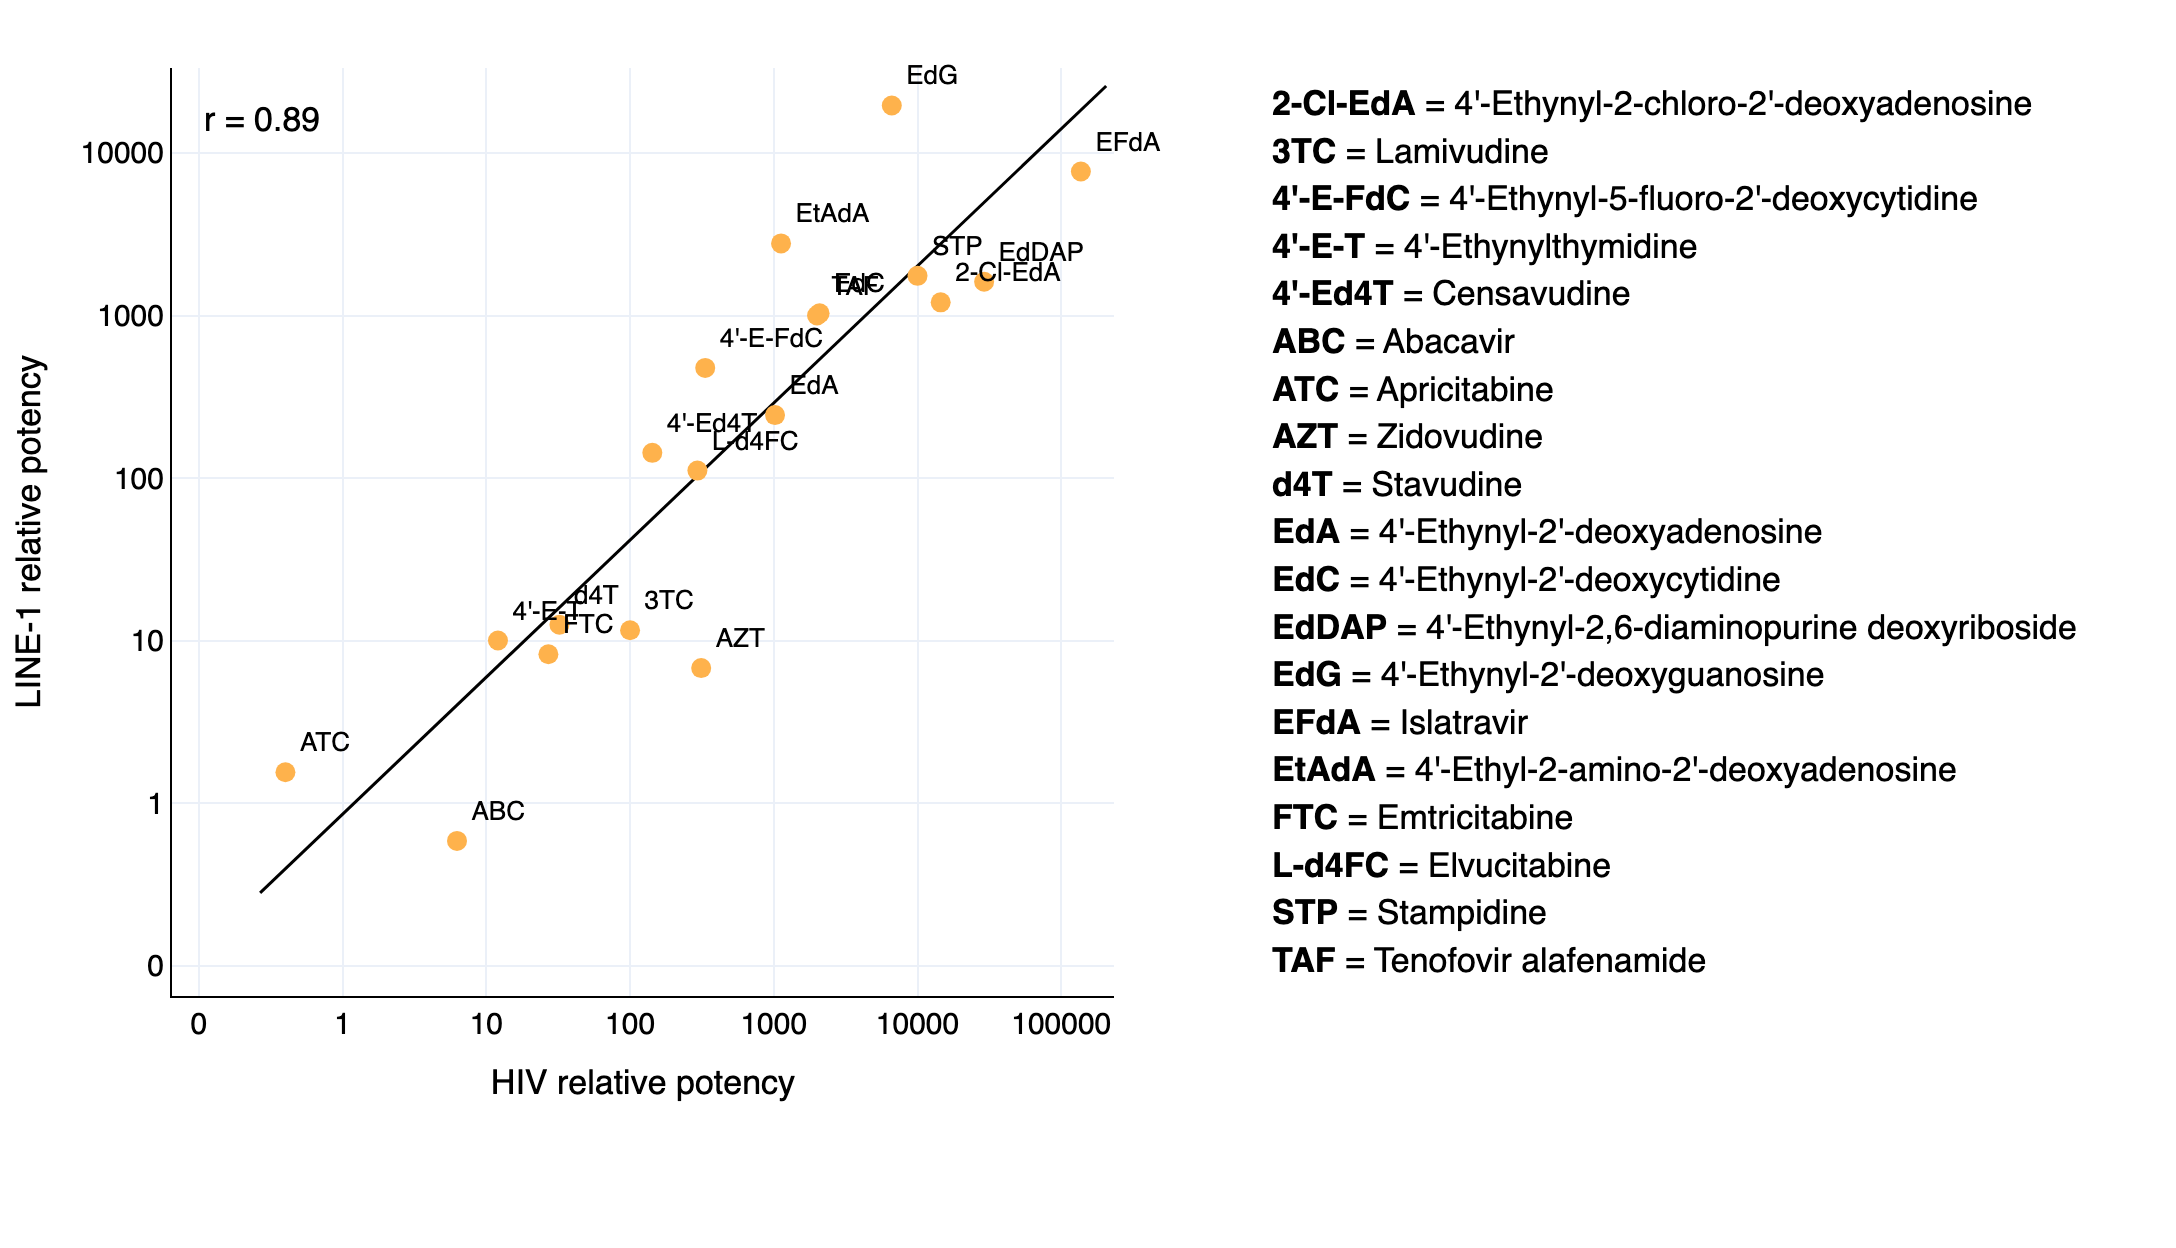
\includegraphics[width=0.877\textwidth]{../line1_hiv_correlation.png}
\end{minipage}
\par\vspace{0.55em}
\noindent
\begin{minipage}[t]{0.306\textwidth}
{\sffamily\bfseries B}\par\vspace{1pt}
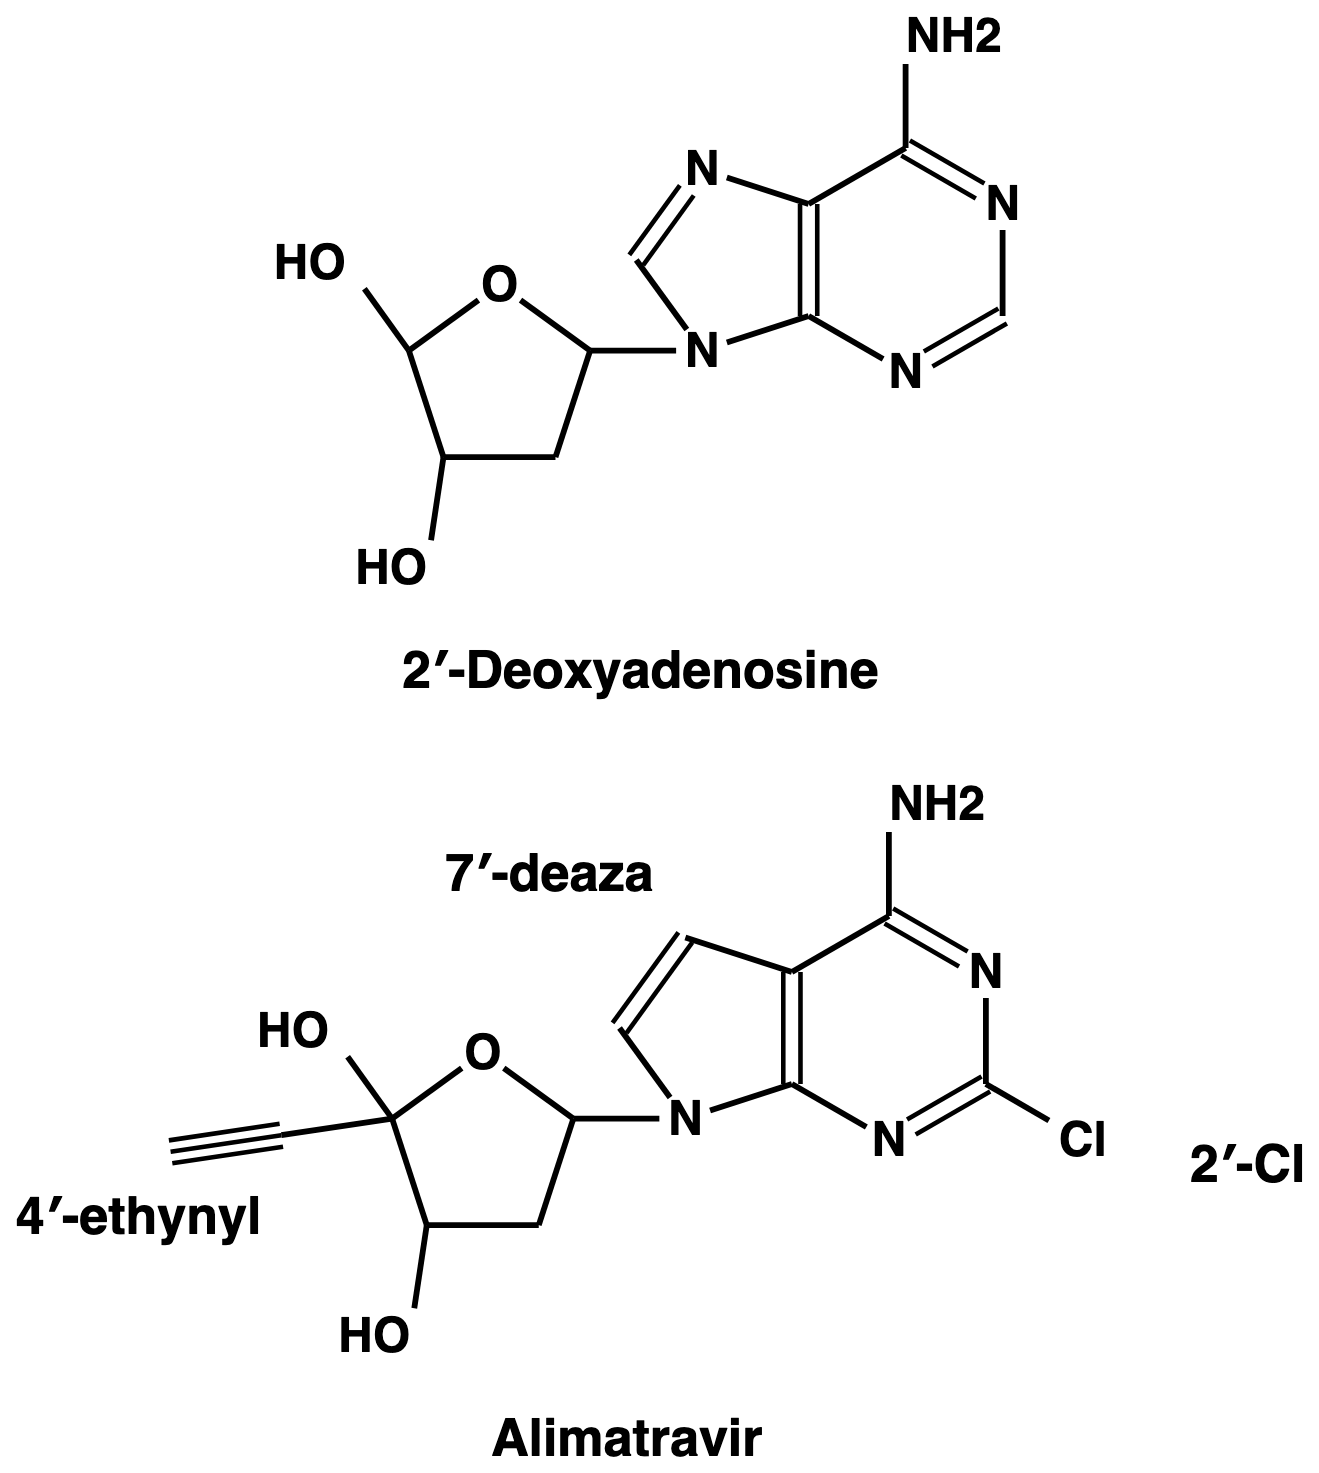
\includegraphics[width=\linewidth]{alimatravir_stacked.png}
\end{minipage}\hfill
\begin{minipage}[t]{0.567\textwidth}
{\sffamily\bfseries C}\par\vspace{1pt}
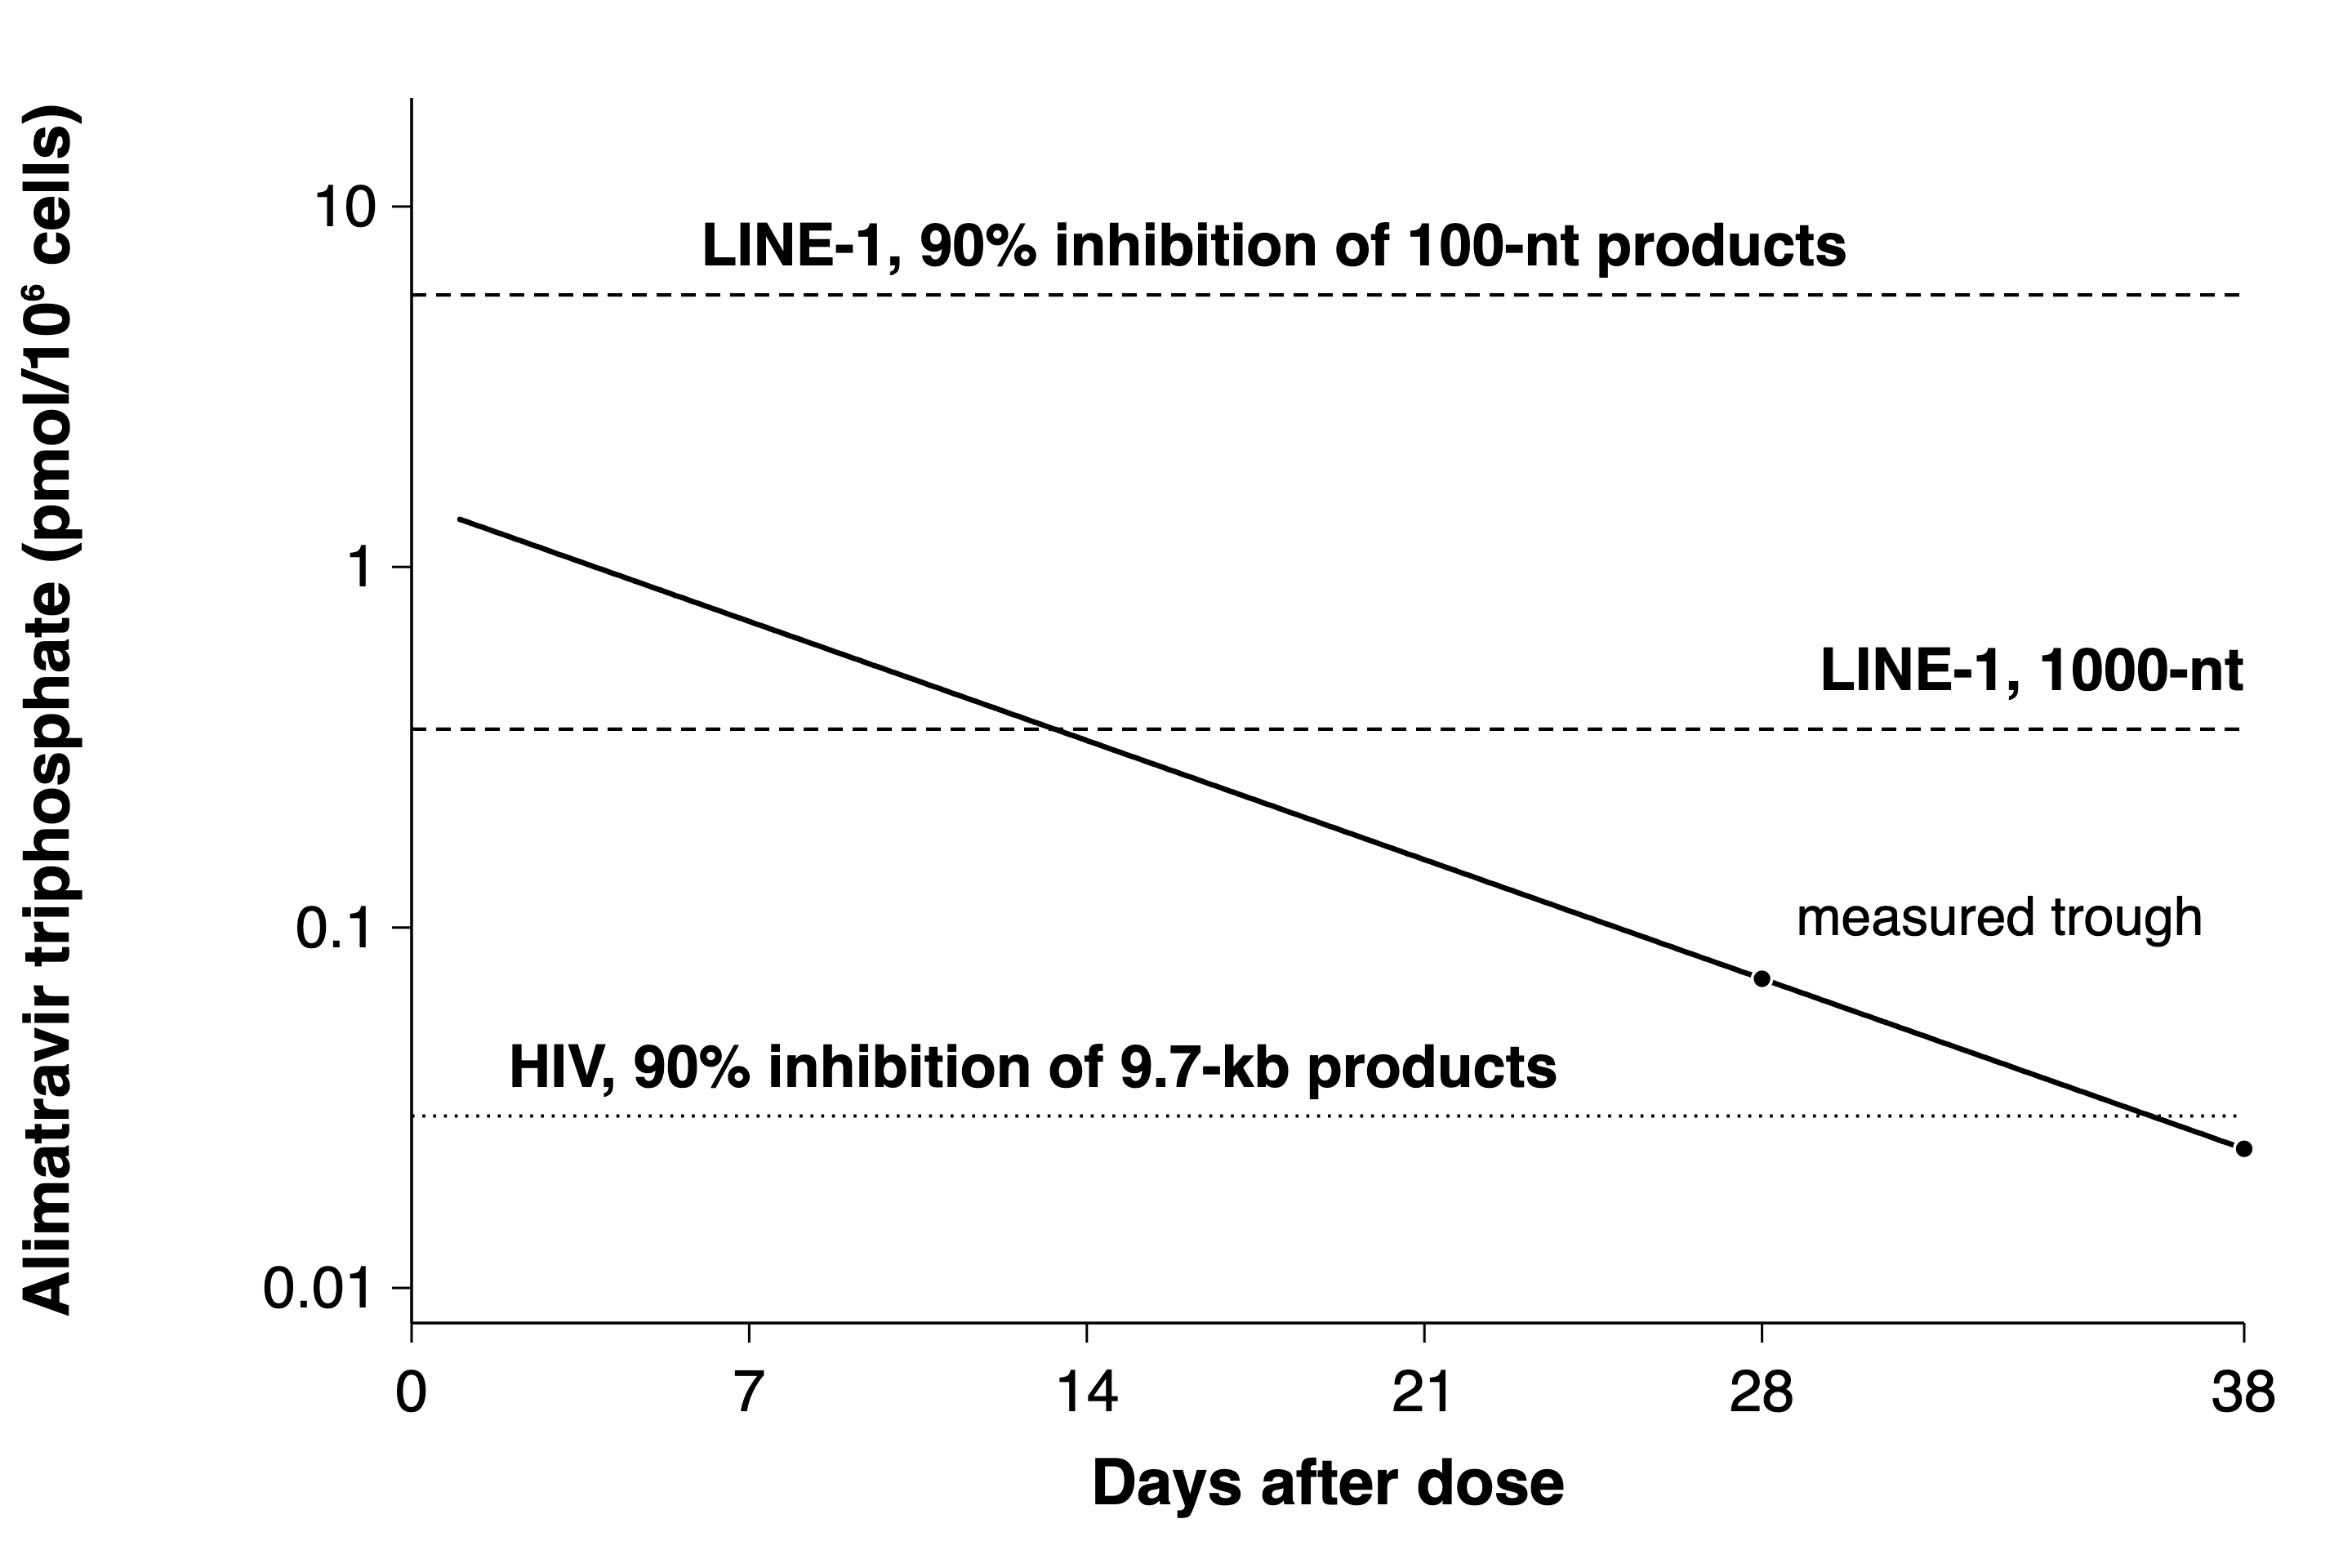
\includegraphics[width=\linewidth]{../alimatravir_11mg_decay.png}
\end{minipage}
\caption{\textbf{Nucleoside potency, structure, and exposure.}
\textbf{a}, Relative potency of nucleoside analogues. LINE-1 potency tracks HIV potency.
\textbf{b}, Deoxyadenosine and alimatravir. Alimatravir is an example reverse transcriptase inhibitor, 2-chloro-7-deaza-4$'$-ethynyl-2$'$-deoxyadenosine.
\textbf{c}, Intracellular alimatravir triphosphate after a monthly 11\,mg oral dose, in pmol per 10$^{6}$ peripheral blood mononuclear cells, on a logarithmic scale. The upper line is the calculated concentration at which 90\% of 100-nt products would be inhibited. The middle line is the same calculation for 1,000-nt products. The LINE-1 IC$_{50}$ is extrapolated from panel A, then scaled by template length. The lower line is the published threshold for 90\% inhibition of a 9.7\,kb HIV product.
Data are from US20240173346A1, US20230293526A1, US20240366649A1, US20260035403A1, US12187758B2, EP1177202B1\cite{raheem,kawamoto,kodama,takamatsu,lin,nitanda,hachiya,parkin,mayer}}
\label{fig:nrti}
\end{figure*}

\begin{table*}[!t]
\caption{\textbf{Example nucleoside analogues tested on LINE-1 and HIV.}
Concentrations are nM}
\label{tab:nucleosides}
\vspace{0.25em}
\scriptsize
\setlength{\tabcolsep}{3.2pt}
\renewcommand{\arraystretch}{1.08}
\centering
\begin{tabular}{@{}>{\raggedright\arraybackslash}p{6.05cm} l c r r r r r r@{}}
\toprule
\textbf{Compound} & \textbf{Short} & \textbf{Base} & \textbf{LINE-1 IC$_{50}$} & \textbf{HIV EC$_{50}$} & \textbf{CC$_{50}$} & \textbf{Pol $\gamma$} & \textbf{Pol $\alpha$} & \textbf{Telomerase} \\
\midrule
Alimatravir & MK-8527 & A &  & 0.21 & $>$42,000 & $>$200,000 & 95,000 &  \\
Islatravir & EFdA & A & 1.3 & 0.073 & 7,500 & 10,000 & $>$100,000 &  \\
4$'$-Ethynyl-2$'$-deoxyguanosine & EdG & G & 0.51 & 1.51 & 1,400 &  &  &  \\
4$'$-Ethynyl-2,6-diaminopurine deoxyriboside & EdDAP & A & 6.2 & 0.344 & 900 &  &  &  \\
4$'$-Ethyl-2-amino-2$'$-deoxyadenosine & EtAdA & A & 3.6 & 8.9 & 35,900 &  &  &  \\
4$'$-Ethynyl-2$'$-deoxycytidine & EdC & C & 9.7 & 4.8 & 2,200 &  &  &  \\
Tenofovir alafenamide & TAF & A & 10 & 5 & 4,700 &  &  & 13,000 \\
ROME compound I-1 & I-1 & A & 8.3 &  & $>$100,000 &  &  &  \\
4$'$-vinyl-5-fluoro-2$'$-deoxycytidine & ROME-74 & C & 9 &  & $>$100,000 &  &  &  \\
4$'$-vinyl-2$'$-deoxyguanosine & ROME-69 & G & 13 &  & $>$1,000--$\leq$10,000 &  &  &  \\
4$'$-Ethynyl-5-fluoro-2$'$-deoxycytidine & 4$'$-E-FdC & C & 21 & 30 & $>$100,000 &  &  &  \\
4$'$-chloromethyl-2$'$-deoxycytidine & ROME-2 & C & $<$50 &  & $>$100,000 & $\leq$50,000 &  & $\leq$1,000 \\
2$'$-fluoro-4$'$-chloromethyl-5-fluoro-2$'$-deoxycytidine & ROME-67 & C & $<$50 &  & $>$100,000 & $>$200,000--$\leq$300,000 &  & $>$100,000 \\
Elvucitabine & L-d4FC & C & 90 & 34 &  &  &  &  \\
Censavudine & 4$'$-Ed4T & T & 70 & 70 & $>$100,000 & 100,000 & $>$100,000 &  \\
Lamivudine & 3TC & C & 640 & 100 & $>$100,000 &  &  & $>$150,000 \\
Zidovudine & AZT & T & 810 & 32 & 29,000 &  &  & 46,000 \\
Stavudine & d4T & T & 750 & 310 & 79,000 & 1,000 &  & 15,000 \\
Emtricitabine & FTC & C & 1,340 & 370 &  &  &  & $>$150,000 \\
4$'$-Ethynylthymidine & 4$'$-E-T & T & $>$1,000 & 830 & $>$400,000 &  &  &  \\
Abacavir & ABC & G & 17,100 & 1,600 &  &  &  & 9,000 \\
\bottomrule
\end{tabular}
\par\vspace{0.35em}
{\raggedright\footnotesize Data are from US20240173346A1, US20230293526A1, US20240366649A1, US20260035403A1, US12187758B2, EP1177202B1\cite{raheem,kawamoto,kodama,takamatsu,lin,nitanda,hachiya,parkin,ohrui,nakata,haraguchi,yangpol,baldwin,callebaut}\par}
\end{table*}

\subsubsection{Adenosine}
Adenosine analogues have specific modifications that prevent their metabolism and increase their selectivity for HIV

Many adenosine analogues have been made, however, we'll just focus on one as an example, Alimatravir, which has a wide therapeutic window and long half-life (2-Chloro-7-deaza-4$'$-ethynyl-2$'$-deoxyadenosine; Table~\ref{tab:nucleosides}; Figure~\ref{fig:nrti}B; Raheem et al., 2025; Michailidis et al., 2009). It is in Phase 3 at 11\,mg monthly for HIV pre-exposure prophylaxis. In peripheral blood cells, that dose is sufficient to keep triphosphate levels above the completed HIV insertion threshold for one month. No other nucleosides have shown sufficient safety or potency to be dosed only once per month. Alimatravir has no published LINE-1 half-maximal inhibitory concentration (IC$_{50}$). However, we can estimate it by extrapolating from Figure~\ref{fig:nrti}A and scaling by template length. Alimatravir may not be sufficient to block 100-nt or 1,000-nt products of LINE-1 throughout monthly dosing (Figure~\ref{fig:nrti}C). More frequent dosing may be required, and the safety of this is not established

There are three modifications to the bare nucleoside of Alimatravir that enable its high therapeutic index and long half-life. A 2-chloro group on the adenine base prevents adenosine deaminase from metabolizing the nucleoside to inosine (Raheem et al., 2025). The 4$'$-ethynyl group on the ribose sugar limits breakdown of the triphosphate by SAMHD1 (Huber et al., 2014), and it is incorporated more selectively into HIV and LINE-1 reverse transcriptase (Michailidis et al., 2009). Finally, the 7-deaza group prevents breakdown by purine nucleoside phosphorylase (Raheem et al., 2025)

Adenine has two positions that can be altered while sparing Watson-Crick base pairing, whereas cytosine and thymine are mostly limited to one position. Both of those positions are also used by catabolic enzymes to break down the nucleoside. Modifying them enables both a longer half-life and selectivity for HIV / LINE-1

Although there is no public measurement of LINE-1 inhibition for Alimatravir, nor data on its ability to cross the blood-brain barrier. We can assume the data will be similar to Islatravir (EFdA; Figure~\ref{fig:nrti}A), another adenosine analogue from the same series as Alimatravir (Stoddart et al., 2015)

\subsubsection{Thymidine}
When LINE-1 is reverse transcribed it starts copying the polyA tail of its messenger RNA, which is $\sim$40 nucleotides long and is complementary to thymidine (Figure~\ref{fig:genomes}). Thymidine analogues therefore could in theory shut down LINE-1 reverse transcription before it is able to contribute to inflammation. Thymidine nucleosides primarily get activated by thymidine kinase 1 (TK1). This enzyme is only present in dividing cells, as thymidine is required only for DNA (not for RNA). Whereas resting cells can synthesize dTTP as needed, rendering thymidine analogues potentially less effective in non-dividing cells such as neurons (Sherley and Kelly, 1988). Thymidine analogues therefore may be particularly beneficial in dividing cells such as in cancer, especially given the chemotherapy standard of care (SoC) leverages thymidine synthesis inhibitors (5-FU), which is rationally synergistic with thymidine analogues

Mitochondria contain their own thymidine kinase, which can activate nucleosides and contribute to mitochondrial toxicity (Arn\'er and Eriksson, 1995). The thymidine analogue censavudine has a 4$'$-ethynyl modification (like Alimatravir), which enables both a strong LINE-1 potency and orders of magnitude lower incorporation into mitochondrial polymerase gamma (Yang et al., 2007)

Unfortunately, the cell efficiently turns over thymidine-triphosphates. Thymidine is also cleared by thymidine phosphorylase cutting its glycosidic bond. Although Censavudine's 4$'$-ethynyl resists this process, its half-life is still much shorter than that of adenosine analogues such as Alimatravir. Censavudine has been used in a Phase 2 trial for amyotrophic lateral sclerosis / frontotemporal dementia (NCT04993755). The ALS functional rating (ALSFRS-R) did not differ from placebo over the 24-week blinded period

\subsubsection{Cytidine}
Two of the most commonly prescribed nucleosides for HIV are cytidine analogues, Lamivudine (3TC) and Emtricitabine (FTC). Although their potency is not as high as for other molecules, they have strong safety records due to having opposite chirality to natural nucleosides, alongside other modifications (Coates et al., 1992). Lamivudine has been tested in a Phase 2 trial for stage IV colorectal cancer (NCT03144804), and showed some suggestion of disease stabilization, but had no control arm (Rajurkar et al., 2022). Lamivudine at standard doses is not potent enough to sufficiently suppress LINE-1. ROME therapeutics screened cytidine nucleosides for LINE-1, generating novel compounds that have greater potency than 3TC or FTC, and which may be in the same range as the adenosine analogues (ROME Therapeutics, US12187758B2; Table~\ref{tab:nucleosides}). However, their safety is not established. It is not known if any are as potent as Alimatravir, as published data had a limit of detection of 50\,nM (Table~\ref{tab:nucleosides}). One advantage cytidine analogues have is they are not incorporated into telomerase because the enzyme adds a fixed TTAGGG repeat (Table~\ref{tab:nucleosides}) and does not use cytidine

\subsubsection{Guanosine}
Guanosine analogues have historically had issues with toxicity. The most potent known nucleoside for LINE-1 is 4$'$-Ethynyl-2$'$-deoxyguanosine (0.51\,nM) (Table~\ref{tab:nucleosides}; Figure~\ref{fig:nrti}A). In six-week-old male mice, one dose of 4$'$-ethynyl-deoxyguanosine also killed every animal at 3 mg/kg within a few days (Ohrui, 2011), but 1 mg/kg did not. In the same experiment, 4$'$-ethynyl-deoxyadenosine was tolerated at 100\,mg/kg. Although highly potent (Figure~\ref{fig:nrti}A), none are approved for HIV. Deoxyguanosine analogues are phosphorylated mainly by mitochondrial deoxyguanosine kinase, which may contribute to toxicity due to proximity to mitochondrial polymerase gamma. Guanosine analogues are underexplored, and like adenosine have two positions on the base that can be modified without impacting Watson-Crick base pairing. However, LINE-1 is AT rich ($\sim$57\%) and adenosine and thymidine analogues appear preferable

\subsubsection{Prodrug formulations}
Bare nucleosides of guanosine, cytidine and adenosine cannot easily be combined because they compete with each other for phosphorylation by cellular kinase enzymes (Arn\'er and Eriksson, 1995). In theory this is less problematic for the potent nucleosides, because the ratio of nucleoside to natural dNTPs is lower. Tenofovir alafenamide (TAF) is a prodrug formulation that contains a phosphonate group that has been masked, enabling combinations of the nucleosides as the first phosphorylation step is not necessary to activate TAF. While potent for HIV and LINE-1 (Callebaut et al., 2015; Table~\ref{tab:nucleosides}), the downside of this approach is the prodrug formulations do not typically cross the blood-brain barrier as well as bare nucleosides (Best et al., 2012). Also adenosines are readily phosphorylated, and both islatravir \& alimatravir are more potent than TAF while being bare nucleosides (Table~\ref{tab:nucleosides})

\subsection{ORF2p non-nucleoside inhibitors}
Even if LINE-1 reverse transcription is completely shut down, this does not prevent LINE-1's ORF2p endonuclease domain from cutting DNA. This is so toxic to cells that scientists were not able to produce enough of the protein to determine its structure until 2023 (Baldwin et al., 2024; Leslie, 2025; Thawani et al., 2024). One attempt has been made to make a non-nucleoside inhibitor that inhibits the endonuclease domain of ORF2p (D'Ordine et al., 2024). One challenge is that the endonuclease shares conserved catalytic sites with host DNA repair enzymes such as APE1. Just like with HIV, a combination of a reverse transcriptase inhibitor with a non-nucleoside small molecule inhibitor may be necessary to shut down LINE-1's activity

\subsection{Antisense Oligonucleotides}
Antisense oligonucleotides (ASOs) could potentially prevent the translation of LINE-1 mRNA into ORF1p \& ORF2p. They have shown promise for LINE-1 in preclinical models of Hutchinson-Gilford progeria (Della Valle et al., 2022) and Alzheimer's (Herdy et al., 2026). However, LINE-1 is 17\% of the genome. All ASO designs for LINE-1 have hundreds of potential off-target effects in introns of pre-mRNA. There are two types of ASO, a gapmer, which is modified RNA nucleotides with a DNA gap that recruits RNase H to cut the bound RNA catalytically, and steric blockers, which occupy the target site, preventing translation. For gapmers, LINE-1 ASOs would also degrade potentially important coding gene transcripts. For steric blockers their effects would be diluted by off-target binding, requiring high doses. Short interfering RNAs (siRNAs) also present similar challenges of off-target effects

\section{Detecting LINE-1 activity in disease}
Having effective inhibitors against LINE-1 is not sufficient. We also need to know under what contexts to administer them. To date more progress has been made in detecting LINE-1 activity in cancer than in other diseases. Tumor cells are clonal, enabling detection of retrotransposons using bulk whole-genome sequencing (Rodriguez-Martin et al., 2020; Cajuso et al., 2019; Zhang et al., 2026; Zumalave et al., 2026; Mendez-Dorantes et al., 2026). Furthermore, dying cancer cells shed proteins such as ORF1p into blood, enabling detection of LINE-1 activity from a blood draw (Taylor et al., 2023)

It is now possible to detect retrotransposons jumping in individual cells through single-nucleus whole-genome sequencing. Although not yet demonstrated for LINE-1, structural variants can be detected in single nuclei, and are detected using similar signatures (Luquette et al., 2025). Bioinformatics tools such as retrotransposon-miner could be adapted to single-nucleus sequencing for this purpose (\href{https://github.com/L1-Therapeutics/retrotransposon-miner}{\faGithub}). Retrotransposon-miner is developed by L1 Therapeutics (\url{https://l1tx.com}). This opens the possibility of sequencing single nuclei from both post-mortem tissue and biopsies to determine what diseases and what time points in a disease are most amenable to LINE-1 inhibitors

\section{Discussion and Future Perspectives}
LINE-1 has fundamentally shaped the structure of the genome over evolutionary time. Because of its effects on the genome, it is heavily suppressed in healthy adult cells. Increasing evidence suggests that this suppression is compromised in various diseases, and also under the stress of certain treatments. This makes it a compelling therapeutic target

The challenge with all diseases where LINE-1 is implicated is that treatment with inhibitors is not likely to be a cure for that disease, instead LINE-1 may slow or stop progression. For example, in cancer LINE-1 causes mutations that can contribute to tumor evolution. But it is not the only source of mutations, and although preclinical studies have shown LINE-1 inhibition can slow tumor cell growth or division, it is not understood how well that would counteract tumor progression in humans. Similar uncertainties remain for degeneration and inflammatory diseases. Most studies in these diseases are preliminary, and we do not have a clear picture of the relative importance of LINE-1 to each disease. New genomics technologies such as single-nucleus whole-genome sequencing enable the quantification of the prevalence of insertions in diseased tissue across a range of ages and disease stages. This would help measure LINE-1's contribution to genome instability, and act as a proxy for its inflammatory effects. Measuring this requires development of novel computational biology algorithms

The potency, safety and low cost of next generation reverse transcriptase inhibitors potentially enable their application to LINE-1. However, this also creates a challenge for expanding access for nucleosides to LINE-1, because the cost of performing the necessary preclinical work and trials to determine safe dosing and when treatment would be effective may exceed what can be recouped due to pricing pressure from off-label prescribing

However, reverse transcriptase inhibitors alone may not be sufficient for LINE-1, even at higher doses. Stopping reverse transcriptase early may free up ORF2p endonuclease to repeatedly cut DNA (Rajurkar et al., 2022). However, this is unlikely given reverse transcriptase inhibitors reduce DNA damage rather than increasing it (D'Ordine et al., 2024). Also, the success of reverse transcriptase inhibitors outside of cancer in preclinical studies argues against this hypothesis

Regardless, a combination of inhibitors may be required for LINE-1 because reverse transcriptase inhibitors only partially prevent DNA damage (D'Ordine et al., 2024). More than 10 DNA cuts are made for each successful insertion (Gasior et al., 2006). A selective inhibitor that blocks endonuclease activity or degrades the protein could provide greater protection against LINE-1 activation. As of October 2026, there is no publicly announced program for novel non-nucleoside inhibitors of ORF2p

LINE-1 is an unconventional target for new medicines. It encodes proteins, but is not a gene. It is virus-like, but not infectious. It is suppressed in healthy adults and has been associated with many diseases, but its contribution to each disease is not firmly established. Evidence increasingly suggests therapeutics for LINE-1 could have broad reach, however we have not established precisely when diseases are therapeutically actionable. This creates both challenges and opportunities for inhibiting LINE-1 therapeutically in disease


\section{Competing interests}
W.B. is founder of L1 Therapeutics. The retrotransposon-miner software cited in this article is developed by L1 Therapeutics

\FloatBarrier
\begin{thebibliography}{99}
\footnotesize
\setlength{\itemsep}{0.12em}
\setlength{\parsep}{0pt}

\bibitem{cecco} De Cecco, M. et al. LINE-1 derepression in senescent cells triggers interferon and inflammaging. \textit{Nature} \textbf{566}, 73--78 (2019) doi:10.1038/s41586-018-0784-9

\bibitem{you} You, E. et al. LINE-1 ORF1p mimics viral innate immune evasion mechanisms in pancreatic ductal adenocarcinoma. \textit{Cancer Discov.} \textbf{15}, 1063--1082 (2025) doi:10.1158/2159-8290.cd-24-1317

\bibitem{rodriguez} Rodriguez-Martin, B. et al. Pan-cancer analysis of whole genomes identifies driver rearrangements promoted by LINE-1 retrotransposition. \textit{Nat. Genet.} \textbf{52}, 306--319 (2020) doi:10.1038/s41588-019-0562-0

\bibitem{gasior} Gasior, S. L., Wakeman, T. P., Xu, B. \& Deininger, P. L. The human LINE-1 retrotransposon creates DNA double-strand breaks. \textit{J. Mol. Biol.} \textbf{357}, 1383--1393 (2006) doi:10.1016/j.jmb.2006.01.089

\bibitem{ivancevic} Ivancevic, A. M., Kortschak, R. D., Bertozzi, T. \& Adelson, D. L. LINEs between Species: Evolutionary Dynamics of LINE-1 Retrotransposons across the Eukaryotic Tree of Life. \textit{Genome Biol. Evol.} \textbf{8}, 3301--3322 (2016) doi:10.1093/gbe/evw243

\bibitem{goodier2001} Goodier, J. L., Ostertag, E. M., Du, K. \& Kazazian, H. H. A novel active L1 retrotransposon subfamily in the mouse. \textit{Genome Res.} \textbf{11}, 1677--1685 (2001) doi:10.1101/gr.198301

\bibitem{mclaughlin} Yang, L. et al. Evolutionary insights from profiling LINE-1 activity at allelic resolution in a single human genome. \textit{EMBO J.} \textbf{43}, 112--131 (2024) doi:10.1038/s44318-023-00007-y

\bibitem{baldwin} Baldwin, E. T. et al. Structures, functions and adaptations of the human LINE-1 ORF2 protein. \textit{Nature} \textbf{626}, 194--206 (2024) doi:10.1038/s41586-023-06947-z

\bibitem{morrish} Morrish, T. A. et al. DNA repair mediated by endonuclease-independent LINE-1 retrotransposition. \textit{Nat. Genet.} \textbf{31}, 159--165 (2002) doi:10.1038/ng898

\bibitem{jacob} Jacob-Hirsch, J. et al. Whole-genome sequencing reveals principles of brain retrotransposition in neurodevelopmental disorders. \textit{Cell Res.} \textbf{28}, 187--203 (2018) doi:10.1038/cr.2018.8

\bibitem{perepelitsa} Perepelitsa-Belancio, V. \& Deininger, P. RNA truncation by premature polyadenylation attenuates human mobile element activity. \textit{Nat. Genet.} \textbf{35}, 363--366 (2003) doi:10.1038/ng1269

\bibitem{cajuso} Cajuso, T. et al. Retrotransposon insertions can initiate colorectal cancer and are associated with poor survival. \textit{Nat. Commun.} \textbf{10}, 4022 (2019) doi:10.1038/s41467-019-11770-0

\bibitem{zhang} Zhang, T. et al. Uncovering the role of LINE-1 in the evolution of lung adenocarcinoma. \textit{Nature} \textbf{650}, 230--241 (2026) doi:10.1038/s41586-025-09825-y

\bibitem{pisanic} Pisanic, T. R. et al. Long interspersed nuclear element 1 retrotransposons become deregulated during the development of ovarian cancer precursor lesions. \textit{Am. J. Pathol.} \textbf{189}, 513--520 (2019) doi:10.1016/j.ajpath.2018.11.005

\bibitem{zumalave} Zumalave, S. et al. Concurrent L1 retrotransposition events promote reciprocal translocations in human tumorigenesis. \textit{Science} \textbf{392}, eaee4513 (2026) doi:10.1126/science.aee4513

\bibitem{mendez} Mendez-Dorantes, C. et al. Chromosomal rearrangements and instability caused by LINE-1 retrotransposition. 2024.12.14.628481 Preprint at \url{https://doi.org/10.1101/2024.12.14.628481} (2026)

\bibitem{goodier2016} Goodier, J. L. Restricting retrotransposons: a review. \textit{Mob. DNA} \textbf{7}, 16 (2016) doi:10.1186/s13100-016-0070-z

\bibitem{leslie} Leslie, M. Risky moves. \textit{Science} \textbf{388}, 244--247 (2025) doi:10.1126/science.ady2285

\bibitem{rajurkar} Rajurkar, M. et al. Reverse Transcriptase Inhibition Disrupts Repeat Element Life Cycle in Colorectal Cancer. \textit{Cancer Discov.} \textbf{12}, 1462--1481 (2022) doi:10.1158/2159-8290.cd-21-1117

\bibitem{novototskaya} Novototskaya-Vlasova, K. A. et al. Inflammatory response to retrotransposons drives tumor drug resistance that can be prevented by reverse transcriptase inhibitors. \textit{Proc. Natl. Acad. Sci. U. S. A.} \textbf{119}, e2213146119 (2022) doi:10.1073/pnas.2213146119

\bibitem{simon} Simon, M. et al. LINE1 Derepression in Aged Wild-Type and SIRT6-Deficient Mice Drives Inflammation. \textit{Cell Metab.} \textbf{29}, 871--885.e5 (2019) doi:10.1016/j.cmet.2019.02.014

\bibitem{dellavalle} Della Valle, F. et al. LINE-1 RNA causes heterochromatin erosion and is a target for amelioration of senescent phenotypes in progeroid syndromes. \textit{Sci. Transl. Med.} \textbf{14}, eabl6057 (2022) doi:10.1126/scitranslmed.abl6057

\bibitem{muotri} Muotri, A. R. et al. L1 retrotransposition in neurons is modulated by MeCP2. \textit{Nature} \textbf{468}, 443--446 (2010) doi:10.1038/nature09544

\bibitem{martins} Martins, A. M. A. et al. Dormant viral pathways underlie space-induced neural senescence. 2025.11.02.686043 Preprint at \url{https://doi.org/10.1101/2025.11.02.686043} (2026)

\bibitem{takahashi} Takahashi, T. et al. LINE-1 activation in the cerebellum drives ataxia. \textit{Neuron} \textbf{110}, 3278--3287.e8 (2022) doi:10.1016/j.neuron.2022.08.011

\bibitem{thomas} Thomas, C. A. et al. Modeling of TREX1-Dependent Autoimmune Disease using Human Stem Cells Highlights L1 Accumulation as a Source of Neuroinflammation. \textit{Cell Stem Cell} \textbf{21}, 319--331.e8 (2017) doi:10.1016/j.stem.2017.07.009

\bibitem{martinez} Martinez de Lagran, M., Elizalde-Torrent, A., Paredes, R., Clotet, B. \& Dierssen, M. Lamivudine, a reverse transcriptase inhibitor, rescues cognitive deficits in a mouse model of down syndrome. \textit{J. Cell. Mol. Med.} \textbf{26}, 4210--4215 (2022) doi:10.1111/jcmm.17411

\bibitem{borgognone} Borgognone, A. et al. Lamivudine modulates the expression of neurological impairment-related genes and LINE-1 retrotransposons in brain tissues of a Down syndrome mouse model. \textit{Front. Aging Neurosci.} \textbf{16}, 1386944 (2024) doi:10.3389/fnagi.2024.1386944

\bibitem{guo} Guo, C. et al. Tau activates transposable elements in Alzheimer's disease. \textit{Cell Rep.} \textbf{23}, 2874--2880 (2018) doi:10.1016/j.celrep.2018.05.004

\bibitem{sun} Sun, W. et al. Pathogenic tau-induced piRNA depletion promotes neuronal death through transposable element dysregulation in neurodegenerative tauopathies. \textit{Nat. Neurosci.} \textbf{21}, 1038--1048 (2018) doi:10.1038/s41593-018-0194-1

\bibitem{herdy} Herdy, J. R. et al. Cytoplasmic DNA Sensing Links LINE-1 Expression to Neuronal Senescence in Alzheimer's Disease. 2026.07.27.740588 Preprint at \url{https://doi.org/10.64898/2026.07.27.740588} (2026)

\bibitem{faulkner} Faulkner, G. J. Elevated L1 expression in ataxia telangiectasia likely explained by an RNA-seq batch effect. \textit{Neuron} \textbf{111}, 610--611 (2023) doi:10.1016/j.neuron.2023.02.007

\bibitem{upton} Upton, K. R. et al. Ubiquitous L1 mosaicism in hippocampal neurons. \textit{Cell} \textbf{161}, 228--239 (2015) doi:10.1016/j.cell.2015.03.026

\bibitem{erwin} Erwin, J. A. et al. L1-associated genomic regions are deleted in somatic cells of the healthy human brain. \textit{Nat. Neurosci.} \textbf{19}, 1583--1591 (2016) doi:10.1038/nn.4388

\bibitem{evrony} Evrony, G. D., Lee, E., Park, P. J. \& Walsh, C. A. Resolving rates of mutation in the brain using single-neuron genomics. \textit{eLife} \textbf{5}, e12966 (2016) doi:10.7554/elife.12966

\bibitem{crow} Crow, Y. J. et al. Reverse transcriptase inhibitors in Aicardi--Gouti\`eres syndrome: A crossover clinical trial. \textit{Dev. Med. Child Neurol.} \textbf{67}, 750--757 (2025) doi:10.1111/dmcn.16199

\bibitem{coufal} Coufal, N. G. et al. Ataxia telangiectasia mutated (ATM) modulates long interspersed element-1 (L1) retrotransposition in human neural stem cells. \textit{Proc. Natl. Acad. Sci.} \textbf{108}, 20382--20387 (2011) doi:10.1073/pnas.1100273108

\bibitem{martin} Martin, K. R. et al. The genomic landscape of tuberous sclerosis complex. \textit{Nat. Commun.} \textbf{8}, 15816 (2017) doi:10.1038/ncomms15816

\bibitem{hwang} Hwang, S.-Y. et al. Human cytomegalovirus harnesses host L1 retrotransposon for efficient replication. \textit{Nat. Commun.} \textbf{15}, 7640 (2024) doi:10.1038/s41467-024-51961-y

\bibitem{park} Park, S., Jeong, J. \& Ahn, K. Human cytomegalovirus infection induces L1 expression through UL38-dependent mTOR-KAP1 pathway. \textit{PLoS ONE} \textbf{20}, e0320512 (2025) doi:10.1371/journal.pone.0320512

\bibitem{bregnard} Br\'egnard, C. et al. Upregulated LINE-1 Activity in the Fanconi Anemia Cancer Susceptibility Syndrome Leads to Spontaneous Pro-inflammatory Cytokine Production. \textit{eBioMedicine} \textbf{8}, 184--194 (2016) doi:10.1016/j.ebiom.2016.05.005

\bibitem{mavragani} Mavragani, C. P. et al. Expression of Long Interspersed Nuclear Element 1 Retroelements and Induction of Type I Interferon in Patients With Systemic Autoimmune Disease. \textit{Arthritis Rheumatol.} \textbf{68}, 2686--2696 (2016) doi:10.1002/art.39795

\bibitem{liu} Liu, E. Y. et al. Loss of Nuclear TDP-43 Is Associated with Decondensation of LINE Retrotransposons. \textit{Cell Rep.} \textbf{27}, 1409--1421.e6 (2019) doi:10.1016/j.celrep.2019.04.003

\bibitem{garza} Garza, R. et al. Activation of transposable elements is linked to a region- and cell-type-specific interferon response in Parkinson's disease. 2025.09.03.673956 Preprint at \url{https://doi.org/10.1101/2025.09.03.673956} (2026)

\bibitem{gordillo} Gordillo-Gonz\'alez, F. et al. A single-cell meta-analysis evidences transposable element dysregulation in sex-based differences in Parkinson's disease. \textit{Neurobiol. Dis.} \textbf{229}, 107580 (2026) doi:10.1016/j.nbd.2026.107580

\bibitem{fukuda} Fukuda, S. et al. Alu complementary DNA is enriched in atrophic macular degeneration and triggers retinal pigmented epithelium toxicity via cytosolic innate immunity. \textit{Sci. Adv.} \textbf{7}, eabj3658 (2021) doi:10.1126/sciadv.abj3658

\bibitem{dordine} D'Ordine, A. M., Jogl, G. \& Sedivy, J. M. Identification and characterization of small molecule inhibitors of the LINE-1 retrotransposon endonuclease. \textit{Nat. Commun.} \textbf{15}, 3883 (2024) doi:10.1038/s41467-024-48066-x

\bibitem{jones} Jones, R. B. et al. Nucleoside Analogue Reverse Transcriptase Inhibitors Differentially Inhibit Human LINE-1 Retrotransposition. \textit{PLOS ONE} \textbf{3}, e1547 (2008) doi:10.1371/journal.pone.0001547

\bibitem{dai} Dai, L., Huang, Q. \& Boeke, J. D. Effect of reverse transcriptase inhibitors on LINE-1 and Ty1 reverse transcriptase activities and on LINE-1 retrotransposition. \textit{BMC Biochem.} \textbf{12}, 18 (2011) doi:10.1186/1471-2091-12-18

\bibitem{mckerrow} McKerrow, W. et al. LINE-1 ORF1p is a shared and immunogenic antigen in cancer. 2025.06.11.659092 Preprint at \url{https://doi.org/10.1101/2025.06.11.659092} (2025)

\bibitem{aiewsakun} Aiewsakun, P. \& Katzourakis, A. Marine origin of retroviruses in the early Palaeozoic Era. \textit{Nat. Commun.} \textbf{8}, 13954 (2017) doi:10.1038/ncomms13954

\bibitem{raheem} Raheem, I. T. et al. MK-8527 is a novel inhibitor of HIV-1 reverse transcriptase translocation with potential for extended-duration dosing. \textit{PLOS Biol.} \textbf{23}, e3003308 (2025) doi:10.1371/journal.pbio.3003308

\bibitem{raheemcroi} Raheem, I. T. et al. Discovery of MK-8527, a long-acting HIV nucleoside reverse transcriptase translocation inhibitor. Conference on Retroviruses and Opportunistic Infections, poster 638 (2024). \url{https://www.croiconference.org/wp-content/uploads/sites/2/posters/2024/638.pdf}

\bibitem{siegel} Siegel, D. et al. Discovery and synthesis of a phosphoramidate prodrug of a pyrrolo[2,1-$f$][1,2,4]triazin-4-amino adenine C-nucleoside (GS-5734) for the treatment of Ebola and emerging viruses. \textit{J. Med. Chem.} \textbf{60}, 1648--1661 (2017) doi:10.1021/acs.jmedchem.6b01594

\bibitem{huber} Huber, A. D. et al. SAMHD1 has differential impact on the efficacies of HIV nucleoside reverse transcriptase inhibitors. \textit{Antimicrob. Agents Chemother.} \textbf{58}, 4915--4924 (2014) doi:10.1128/AAC.02745-14

\bibitem{michailidis} Michailidis, E. et al. Mechanism of inhibition of HIV-1 reverse transcriptase by 4$'$-Ethynyl-2-fluoro-2$'$-deoxyadenosine triphosphate, a translocation-defective reverse transcriptase inhibitor. \textit{J. Biol. Chem.} \textbf{284}, 35681--35691 (2009) doi:10.1074/jbc.m109.036616

\bibitem{stoddart} Stoddart, C. A. et al. Oral administration of the nucleoside EFdA (4$'$-ethynyl-2-fluoro-2$'$-deoxyadenosine) provides rapid suppression of HIV viremia in humanized mice and favorable pharmacokinetic properties in mice and the rhesus macaque. \textit{Antimicrob. Agents Chemother.} \textbf{59}, 4190--4198 (2015) doi:10.1128/aac.05036-14

\bibitem{andreeva} Andreeva, L. et al. cGAS senses long and HMGB/TFAM-bound U-turn DNA by forming protein--DNA ladders. \textit{Nature} \textbf{549}, 394--398 (2017) doi:10.1038/nature23890

\bibitem{du} Du, M. \& Chen, Z. J. DNA-induced liquid phase condensation of cGAS activates innate immune signaling. \textit{Science} \textbf{361}, 704--709 (2018) doi:10.1126/science.aat1022

\bibitem{luecke} Luecke, S. et al. cGAS is activated by DNA in a length-dependent manner. \textit{EMBO Rep.} \textbf{18}, 1707--1715 (2017) doi:10.15252/embr.201744017

\bibitem{mankan} Mankan, A. K. et al. Cytosolic RNA:DNA hybrids activate the cGAS--STING axis. \textit{EMBO J.} \textbf{33}, 2937--2946 (2014) doi:10.15252/embj.201488726

\bibitem{sherley} Sherley, J. L. \& Kelly, T. J. Regulation of human thymidine kinase during the cell cycle. \textit{J. Biol. Chem.} \textbf{263}, 8350--8358 (1988) doi:10.1016/s0021-9258(18)68484-4

\bibitem{arner} Arn\'er, E. S. J. \& Eriksson, S. Mammalian deoxyribonucleoside kinases. \textit{Pharmacol. Ther.} \textbf{67}, 155--186 (1995) doi:10.1016/0163-7258(95)00015-9

\bibitem{coates} Coates, J. A. et al. ($-$)-2$'$-deoxy-3$'$-thiacytidine is a potent, highly selective inhibitor of human immunodeficiency virus type 1 and type 2 replication in vitro. \textit{Antimicrob. Agents Chemother.} \textbf{36}, 733--739 (1992) doi:10.1128/aac.36.4.733

\bibitem{ohrui} Ohrui, H. Development of modified nucleosides that have supremely high anti-HIV activity and low toxicity and prevent the emergence of resistant HIV mutants. \textit{Proc. Jpn. Acad. Ser. B Phys. Biol. Sci.} \textbf{87}, 53--65 (2011) doi:10.2183/pjab.87.53

\bibitem{callebaut} Callebaut, C., Stepan, G., Tian, Y. \& Miller, M. D. In Vitro Virology Profile of Tenofovir Alafenamide, a Novel Oral Prodrug of Tenofovir with Improved Antiviral Activity Compared to That of Tenofovir Disoproxil Fumarate. \textit{Antimicrob. Agents Chemother.} \textbf{59}, 5909--5916 (2015) doi:10.1128/aac.01152-15

\bibitem{best} Best, B. M. et al. Low CSF Concentrations of the Nucleotide HIV Reverse Transcriptase Inhibitor, Tenofovir. \textit{J. Acquir. Immune Defic. Syndr. 1999} \textbf{59}, 376--381 (2012) doi:10.1097/qai.0b013e318247ec54

\bibitem{thawani} Thawani, A., Florez Ariza, A. J., Nogales, E. \& Collins, K. Template and target-site recognition by human LINE-1 in retrotransposition. \textit{Nature} \textbf{626}, 186--193 (2024) doi:10.1038/s41586-023-06933-5

\bibitem{kawamoto} Kawamoto, A. et al. 2$'$-Deoxy-4$'$-C-ethynyl-2-halo-adenosines active against drug-resistant human immunodeficiency virus type 1 variants. \textit{Int. J. Biochem. Cell Biol.} \textbf{40}, 2410--2420 (2008) doi:10.1016/j.biocel.2008.04.007

\bibitem{kodama} Kodama, E. N. et al. 4$'$-Ethynyl nucleoside analogs: potent inhibitors of multidrug-resistant human immunodeficiency virus variants in vitro. \textit{Antimicrob. Agents Chemother.} \textbf{45}, 1539--1546 (2001) doi:10.1128/aac.45.5.1539-1546.2001

\bibitem{nakata} Nakata, H. et al. Activity against human immunodeficiency virus type 1, intracellular metabolism, and effects on human DNA polymerases of 4$'$-ethynyl-2-fluoro-2$'$-deoxyadenosine. \textit{Antimicrob. Agents Chemother.} \textbf{51}, 2701--2708 (2007) doi:10.1128/aac.00277-07

\bibitem{takamatsu} Takamatsu, Y. et al. The high genetic barrier of EFdA/MK-8591 stems from strong interactions with the active site of drug-resistant HIV-1 reverse transcriptase. \textit{Cell Chem. Biol.} \textbf{25}, 1268--1278.e3 (2018) doi:10.1016/j.chembiol.2018.07.014

\bibitem{lin} Lin, T.-S. et al. Design and synthesis of 2$'$,3$'$-dideoxy-2$'$,3$'$-didehydro-$\beta$-L-cytidine and 2$'$,3$'$-dideoxy-2$'$,3$'$-didehydro-$\beta$-L-5-fluorocytidine, potent inhibitors of human immunodeficiency virus in vitro. \textit{J. Med. Chem.} \textbf{39}, 1757--1759 (1996) doi:10.1021/jm950836q

\bibitem{nitanda} Nitanda, T. et al. Anti-human immunodeficiency virus type 1 activity and resistance profile of 2$'$,3$'$-didehydro-3$'$-deoxy-4$'$-ethynylthymidine in vitro. \textit{Antimicrob. Agents Chemother.} \textbf{49}, 3355--3360 (2005) doi:10.1128/aac.49.8.3355-3360.2005

\bibitem{haraguchi} Haraguchi, K. et al. From the chemistry of epoxy-sugar nucleosides to the discovery of anti-HIV agent 4$'$-ethynylstavudine-Festinavir. \textit{Curr. Pharm. Des.} \textbf{19}, 1880--1897 (2013) doi:10.2174/1381612811319100011

\bibitem{yangpol} Yang, G. et al. Highly selective action of triphosphate metabolite of 4$'$-ethynyl D4T: a novel anti-HIV compound against HIV-1 RT. \textit{Antiviral Res.} \textbf{73}, 185--191 (2007) doi:10.1016/j.antiviral.2006.10.002

\bibitem{hachiya} Hachiya, A. et al. Evaluation of combinations of 4$'$-ethynyl-2-fluoro-2$'$-deoxyadenosine with clinically used antiretroviral drugs. \textit{Antimicrob. Agents Chemother.} \textbf{57}, 4554--4558 (2013) doi:10.1128/aac.00283-13

\bibitem{parkin} Parkin, N. T. et al. Natural variation of drug susceptibility in wild-type human immunodeficiency virus type 1. \textit{Antimicrob. Agents Chemother.} \textbf{48}, 437--443 (2004) doi:10.1128/aac.48.2.437-443.2004

\bibitem{mayer} Mayer, K. H. et al. Alimatravir oral once monthly in adults with low likelihood of HIV exposure: a randomized, double-blind, placebo-controlled study. \textit{J. Infect. Dis.} (2026) doi:10.1093/infdis/jiag439

\bibitem{taylor} Taylor, M. S. et al. Ultrasensitive detection of circulating LINE-1 ORF1p as a specific multicancer biomarker. \textit{Cancer Discov.} \textbf{13}, 2532--2547 (2023) doi:10.1158/2159-8290.cd-23-0313

\bibitem{luquette} Luquette, L. J. et al. A comprehensive view of somatic mosaicism by single-cell DNA analysis. 2025.10.31.685648 Preprint at \url{https://doi.org/10.1101/2025.10.31.685648} (2025)

\end{thebibliography}

\end{document}
